% RMIT University School of CS&IT
% Minor thesis template
% S.M.M. (Saied) Tahaghoghi, 2004

\documentclass[11pt,twoside]{report}
\usepackage{a4wide,caption,epsfig,fancyheadings,url}
\usepackage{graphicx}
\graphicspath{ {./Figs/} }
\setcounter{secnumdepth}{3}

% Place the correct values here
%Set to the original submission date when submitted amended thesis
\newcommand{\SubmissionDate}{\today}
\newcommand{\student}{Tyler Saxton}
\newcommand{\supervisor}{Dhirendra Singh}
\newcommand{\topic}{Mapping suburban bicycle lanes using street scene images and deep learning}
\newcommand{\school}{School of Computer Science and Information Technology}
\newcommand{\program}{Masters of Data Science}
\newcommand{\institution}{Royal Melbourne Institute of Technology}

% Use the remark command to highlight text for discussion
\newcommand{\remark}[1]{{\bf \em [\marginpar{$\Leftarrow$}#1]}}

\renewcommand{\leftmark}{\student}
\renewcommand{\rightmark}{\topic}
\renewcommand{\headrulewidth}{0pt}
\setlength{\parindent}{0pt}
\setlength{\parskip}{1.5ex plus 0.3ex}

% This is the line spacing - set to 2 for draft submission to
% supervisor, 1.3 for the final submission
\renewcommand{\baselinestretch}{1.3}

\renewcommand{\captionfont}{\it}
\raggedbottom

\begin{document}

%%%%%%%%%%%%%%%%%%%%%%%%%%%%%%%%%%%%%%%%%%%%%%%%%%%%%%%%%%%%%%%%%%%%%%
\title{{\Large\bf \topic}}
\author{
A minor thesis submitted in partial fulfilment of the requirements for the degree of
\\\program\\*[10mm]
%\epsfig{figure=Figs/rmit-coa.epsf,width=5cm}
\\\student
\\\school
\\Science, Engineering, and Technology Portfolio,
\\\institution
\\Melbourne, Victoria, Australia
}
\maketitle
\thispagestyle{empty}


%%%%%%%%%%%%%%%%%%%%%%%%%%%%%%%%%%%%%%%%%%%%%%%%%%%%%%%%%%%%%%%%%%%%%%
\chapter*{Declaration}

This thesis contains work that has not been submitted previously, in
whole or in part, for any other academic award and is solely my
original research, except where acknowledged.

This work has been carried out since March 2021, under the
supervision of {\supervisor}.

\paragraph{}
\vspace{5cm}\noindent \\\student \\
\school\\
\institution\\
\SubmissionDate

\pagenumbering{roman}

%%%%%%%%%%%%%%%%%%%%%%%%%%%%%%%%%%%%%%%%%%%%%%%%%%%%%%%%%%%%%%%%%%%%%%
\chapter*{Acknowledgements}

First and foremost, I would like to thank Dr. Dhirendra Singh for inspiring this research and supervising me throughout the year.  I also greatly appreciate the input provided by Dr. Ron van Schyndel and the ``Research Methods'' class of Semester 1 2021, as I worked to develop a detailed research proposal. \\

To Dr. Sophie Bittinger, Dr. Logan Bittinger, Laura Pritchard, and Dr. Curtis Saxton, thank you for your encouragement, and your assistance with the editing process.



%%%%%%%%%%%%%%%%%%%%%%%%%%%%%%%%%%%%%%%%%%%%%%%%%%%%%%%%%%%%%%%%%%%%%%
\chapter*{To-Do}

\begin{itemize}
\item{Revisit abstract to update the scope of results based on any other suburbs tested}
\item{Repetitive language between Summary and Abstract ``this thesis presents''}
\item{I'm sure I had a better paper on road boundary detection, find it!}
\item{Thesis examples have ``Contribution'' and ``Organisation'' sections}
\item{Insert example GSV detection image}
\item{Picture of some false positive examples}
\item{Picture of the mask}
\item{I have not explained detection confidence threshold}
\item{Example papers using Canny-Hough}
\item{How well do the summary and abstract tie to all four research questions?}
\end{itemize}

%%%%%%%%%%%%%%%%%%%%%%%%%%%%%%%%%%%%%%%%%%%%%%%%%%%%%%%%%%%%%%%%%%%%%%
\chapter*{Summary}

Many policy makers around the world wish to encourage cycling, for health, environmental, and economic reasons.  One significant way they can do this is by providing appropriate infrastructure, including formal on-road bicycle lanes.  It is important for policy makers to have access to accurate information about the existing bicycle network, in order to plan and prioritise upgrades.  Cyclists also benefit when good maps of the bicycle network are available to help them to plan their routes.  This thesis presents an approach to constructing a map of all bicycle lanes within a local area, based on computer analysis of street scene  images sourced from Google Street View or ``dash cam'' footage.

% https://tex.stackexchange.com/questions/131460/remove-pagebreak-after-a-chapter-only-for-one-chapter
\begingroup
\renewcommand{\cleardoublepage}{}
\renewcommand{\clearpage}{}
\chapter*{Abstract}
\endgroup

On-road bicycle lanes improve safety for cyclists, and encourage participation in cycling for active transport and recreation.  With many local authorities responsible for the infrastructure, official maps and datasets of bicycle lanes may be out-of-date and incomplete.  Even ``crowdsourced'' databases may have significant gaps, especially outside popular metropolitan areas.  This thesis presents a method to create a map of bicycle lanes in a local area by taking sample street scene images from each road,  and then applying a deep learning model that has been trained to recognise bicycle lane symbols.  The list of coordinates where bicycle  lanes were detected is then correlated to geospatial data about the road network to record bicycle lane routes.  The method was applied to successfully build a map for a local area in the outer suburbs of Melbourne.  It was able to identify bicycle lanes not previously recorded in the official State government dataset, OpenStreetMap, or the ``biking'' layer of Google Maps.

%%%%%%%%%%%%%%%%%%%%%%%%%%%%%%%%%%%%%%%%%%%%%%%%%%%%%%%%%%%%%%%%%%%%%%

\tableofcontents
\listoffigures
\listoftables


%%%%%%%%%%%%%%%%%%%%%%%%%%%%%%%%%%%%%%%%%%%%%%%%%%%%%%%%%%%%%%%%%%%%%%
\chapter{Introduction}
\pagenumbering{arabic}

\remark{Criteria 15: clear research questions/aims/hypotheses}

\remark{Criteria 15: background knowledge}

The benefits of ``active transport'', such as walking and cycling, have been well documented in previous studies.  Participants' health may improve due to their increased physical activity.  There are environmental benefits due to reduced emissions and pollution.  And there are economic benefits, including a reduced burden on the health system, and reduced transportation costs for participants \cite{LEE2012219} \cite{RABL2012121}.

Federal and State government policy makers in Australia therefore wish to encourage cycling \cite{federal_policy_2019} \cite{state_policy_2020}.  However, the share of cycling for trips to work in Melbourne is only 1.5\% \cite{melbactive}.  For many commuters, a perceived lack of safety of cycling is a major barrier to adoption.  Other significant factors are the availability of shared bicycle schemes and storage facilities, and the risk of theft \cite{WILSON2018234}.  Cycling infrastructure has a significant impact on real and perceived cyclist safety, and this research project will focus on that issue.  Important safety factors include the presence and width of a bicycle lane, the presence of on-street parking, downhill and uphill grades, and the quality of the road surface \cite{BIKESAFETY} \cite{Teschke2012}.  A comprehensive dataset of cycling infrastructure would help policy makers identify and prioritize areas in need of improvement to safety.

In Victoria, Australia, the State government publishes a ``Principal Bicycle Network'' dataset to assist with planning \cite{PrincipalBicycleNetwork}, however it does not appear to be up-to-date.  Individual Local Government Areas may produce their own maps of bicycle routes, but availability is inconsistent \cite{vicroads_maps}.

The aim of this research project was to investigate whether it is possible to construct a dataset or map of bicycle lanes in a local area, by collecting street scene images at known coordinates, and then using a ``deep learning'' machine learning model to detect locations where bicycle lanes are found.  If a baseline map of bicycle lanes can be built in this way, then the process could be extended in future to gather information about other significant factors, such as how frequently the bicycle lane is obstructed by parked vehicles, or the presence of debris or damage to the road surface.

Google Street View has been chosen as a source of street scene image data due to its wide geographical coverage, and the accessibility of the data via a public API.  However, a significant limiting factor is that the Google Street View images for any given location might be several years out of date.  Therefore, the use of images collected from a ``dash cam'' was also explored.  A local government that is responsible for building and maintaining bicycle lanes could use dash cameras to gather its own images, at regular intervals, for more up-to-date data.

\section{Research Questions}
\begin{itemize}
\item{RQ1: Can a ``deep learning'' machine learning model be used to identify on-road bicycle lanes in street scene images sourced from Google Street View?}
\item{RQ2: Can the model then be used to detect and map bicycle lane routes across all streets in a local area with Google Street View coverage?}
\item{RQ3: Can a similar process be applied map bicycle lane routes from street scene images collected from dash camera video footage in a survey area?}
\item{RQ4: Can the approach used to map bicycle lane routes be re-used to visually survey other details about the infrastructure?}
\end{itemize}


%%%%%%%%%%%%%%%%%%%%%%%%%%%%%%%%%%%%%%%%%%%%%%%%%%%%%%%%%%%%%%%%%%%%%%
\chapter{Literature Review}

\remark{Criteria 15: literature review places research in context}

\remark{Criteria 15: background knowledge}

% ~~~~~~~~~~~~~~~~~~~~~~~~~~
\section{Motivation}

Prior research has clearly shown health, economic, and environmental benefits from active transport.  Lee et al., 2012 \cite{LEE2012219} analysed World Health Organization survey data from 2008, and showed that physical inactivity significantly increased the relative risk of coronary heart disease, type 2 diabetes, breast cancer, colon cancer, and all-cause mortality, across dozens of countries.  Rabl \& de Nazelle, 2012 \cite{RABL2012121} demonstrated that active transport by walking or cycling improves those relative risks for participants.  Moderate to vigorous cycling activity for 5 hours a week reduced the all-cause mortality relative risk by more than 30\%.  They estimated an economic gain from improved participant health and reduced pollution, offset slightly by the cost of cycling accidents.

In Australia, Federal and State governments are committed to the principle of supporting active transport through the provision of cycling infrastructure, declaring their commitment through public statements on their official websites \cite{federal_policy_2019} \cite{state_policy_2020}.  Many other governments around the world have adopted similar policies.

Taylor \& Thompson, 2019 \cite{melbactive} surveyed the use of active transport in Melbourne, to establish a baseline of current commuter behaviour.  They found that cycling only accounted for 1.5\% of trips to work in the area.  It could therefore be argued that there is room for improvement.

Schepers et al., 2015 \cite{SCHEPERS2015460} produced a summary of literature related to cycling infrastructure and how it can encourage active transport, resulting in the aforementioned benefits.  The paper found that providing cycling infrastructure that is perceived as being safer does encourage participation.  Other papers such as Wilson et al., 2018 \cite{WILSON2018234} agreed.

Other researchers have examined which factors affect the perceived and actual safety of cycling routes, in a variety of settings.

Klobucar \& Fricker, 2007 \cite{BIKESAFETY} surveyed a group of cyclists in Indiana, USA, asking them to ride a particular route and rate the safety of each road segment along the route, then asking them to review video footage of other routes and rate the safety of those routes, too.  A regression model was created to predict the cyclists' likely safety ratings for other routes.  The creation of the model led to a list of road segment characteristics that were apparently most influential in the area.

Tescheke et al., 2012 \cite{Teschke2012} surveyed patients who attended hospital emergency rooms in Toronto and Vancouver in Canada, due to their involvement in a cycling accident.  Details of the circumstances of each accident were gathered, along with the outcomes.  The data was analysed to determine which factors increased (or decreased) the relative odds of a cyclist being involved in an accident.

Malik et al., 2021 \cite{Malik2021} modelled cyclist safety in Tyne and Wear County in north-east England, a more rural setting.

The factors that contribute to cyclist safety vary by locality.  For example, cyclists in one city might be concerned by the hazard of tram tracks, whereas this might not be a relevant concern in another city, or a less built-up area.  The common themes among the aforementioned papers were:
\begin{itemize}
\item{Presence and type of bicycle lane (dedicated, paved shoulder, none)}
\item{Width of bicycle lane}
\item{Presence of on-street parking}
\item{Downhill or uphill grades}
\item{Volume, speed, and vehicle type profile of motor vehicle traffic}
\item{Quality of road surface (including drainage, tram tracks, etc.)}
\item{Lighting}
\item{Construction Work}
\end{itemize}
Most of these factors can be influenced by infrastructure and road design.  Therefore, it would be valuable to quantify as many of these factors as possible in a dataset, to assist policy makers in deciding what changes ought to be made, and where, to provide a safer network of cycling infrastructure.

% ~~~~~~~~~~~~~~~~~~~~~~~~~~
\section{Applications of Machine Learning}

``Deep Learning'' is a paradigm by which computational models can be constructed to tackle many problems, including visual object recognition.  A Deep Learning model can be trained to perform visual object recognition tasks by supplying it with a ``training'' dataset of images where the objects it must recognise have been pre-labelled.  During training, the model processes its training dataset over and over again, and with each iteration the weights in its multi-layer neural network are refined through the use of a ``backpropagation'' algorithm \cite{deeplearning}.  With a sufficient number of training ``epochs'', the model hopefully develops the ability to detect where the objects of interest appear in each image, to an acceptable level of performance.

Tensorflow \cite{TENSORFLOW2016A} \cite{TENSORFLOW2016B} and PyTorch \cite{pytorch} are two dominant frameworks for building, training, evaluating, and applying Deep Learning models.  Within these frameworks, researchers have progressively developed new models for visual object recognition, typically with a focus on either improving the accuracy of the results, increasing speed to allow ``real time'' processing of video streams, or creating models that will work on low-cost hardware.  Significant Deep Learning models considered within this research project include:

\begin{itemize}
\item{Ren et al., 2015 \cite{REN2016} R-CNN}
\item{Liu et al., 2016 \cite{ssd} SSD}
\item{He et al., 2016 \cite{He_2016_CVPR} ResNet}
\item{Redmon et al., 2016 \cite{YOLOv1} YOLO (and subsequent variants)}
\item{Sandler et al., 2018 \cite{MobileNetV2} MobileNetV2}
\item{Duan et al, 2019 \cite{centernet} CenterNet}
\end{itemize}

The Tensorflow 2 Model Garden \cite{zoo} provides access to many of these models, pre-trained on the COCO 17 (``Microsoft COCO: Common Objects in Context'') dataset.  It therefore provides a convenient library of Deep Learning models that have already received a significant amount of training for the general problem of visual object recognition, and can be re-used to recognise new classes of objects through a process of ``transfer learning'' \cite{coco} \cite{transferlearning}.

Semantic image segmentation of street scene images is an important and active area of computer science research.  ``Deep Learning'' models that can understand sequences of images in real time are essential for self-driving vehicles or similar driver-assistance systems, so many papers have focussed on that area.  In order to train a Deep Learning model that specializes in understanding street scene images, a training dataset of street scene images is required.  Papers by Cordts et al., 2016 \cite{Cordts_2016_CVPR} and Zhou et al., 2019 \cite{ade20k} announced the publication of the ``Cityscapes'' and ``ade20k'' image datasets, respectively.  These datasets each contain many street scene images, with objects of interest labelled in a format suitable for training deep learning models to understand similar on-road scenarios.  Many papers have used these datasets in order to train new machine learning models.  Chen et al., 2018 \cite{DEEPLAB} is one example of a heavily-cited paper where ``CityScapes'' data has been used to train a ``real time'' model to understand street scene images.  Unfortunately, neither of the datasets has cycling infrastructure labelled.  The ``CityScapes'' dataset has labelled bicycle lanes under the ``sidewalks'' category.  This is useful to train a car not to drive there, but a cyclist might not be legally allowed to ride on a sidewalk designed for pedestrian traffic.  

In another branch of research, deep learning tools have been used to manage roadside infrastructure and assets.  Campbell et al., 2019 \cite{CAMPBELL2019101350} used an ``SSD MobileNet'' model to detect ``Stop'' and ``Give Way'' signs on the side of the road in Google Street View images, to help build a database of road sign assets.  An application called ``RectLabel'' was used to label 500 sample images for each type of sign.  Photogrammetry was used to estimate a location for each detected sign, based on the Google Street View camera's position and optical characteristics and the bounding box of the detected sign.  Zhang et al., 2018 \cite{s18082484} performed a similar exercise, detecting road-side utility poles using a ``ResNet'' model.

In Australia, the ``Supplement to Australian Standard AS 1742.9:2000'' sets out the official standards for how bicycle lanes must be constructed and marked.  Generally, a lane marking depicting a bicycle should be painted on the road inside the bicycle lane within 15 metres before and after each intersection, and at 200m intervals \cite{standards}.  Therefore, a Deep Learning model could be trained to detect these markings, similar to how Campbell et al., 2019 \cite{CAMPBELL2019101350} trained a model to detect road signs, and Zhang et al., 2018 \cite{s18082484} trained a model to detect utility poles, using pre-trained models from the TensorFlow 2 Model Garden \cite{zoo} as a starting point.

The use of satellite imagery and aerial photographs were also considered.  Li et al., 2016 \cite{ROADNETWORK} showed that a road network could be extracted from satellite imagery using a convolutional neural network (CNN), and this is particularly useful in rural areas where maps are not already available.  However the resolution of publicly available satellite image data would not be sufficient to identify a bicycle lane on a road, and it would not be able to distinguish a standard bicycle lane from a wide paved shoulder.  Satellite imagery may have a role to play in detecting off-street bicycle tracks in ``green'' parkland area, but it was decided to exclude off-street routes from the scope of this research.

Aerial photography may be useful, where it is available with sufficient detail.  However it would require a different data source for every jurisdiction.  Ning et al., 2021 \cite{NING2021} had success extracting sidewalks from local aerial photography using a ``YOLACT'' model.  Areas of uncertainty caused by tree cover were filled in using Google Street View images.  The model appeared to rely on a concrete sidewalk having a very different colour to the adjacent bitumen road.  The approach might not be able to distinguish bitumen bicycle lanes.  The road markings were not visible.

Aside from formal bicycle lanes, cyclist safety can also be improved by an informal wide paved shoulder, or by creating lanes that are wide enough to safely accommodate a vehicle passing a cyclist.  It may be possible to detect and map these arrangements by recognising lane markings and road boundaries.  A common method of detecting lane boundaries is through the combination of a Canny edge detector \cite{canny} and a Hough transformation \cite{hough}.  The OpenCV library provides a frequently used implementation \cite{opencv}.  Where the Canny-Hough approach struggles with a poorly defined road boundary or ``noise'' from roadside objects, a Deep Learning approach may help:  Mamidala et al., 2019 \cite{8929655} used a ``CNN'' model to detect the outer boundary of roads in Google Street View images.

During the literature review, one other paper was identified where the authors had applied Deep Learning techniques in the domain of cyclist safety:  Rita, 2020 \cite{rita_2020} used the ``MS Coco'' and ``CityScapes'' datasets to train ``YOLOv5'' and ``PSPNet101'' models to identify various classes of object (Bicycle, Car, Truck, Fire Hydrant, etc.) in Google Street View images of London.  A matrix of correlations between objects was calculated.  This was used to infer the circumstances where cyclists might feel the most safe.  For example, there was a high correlation between ``Person'' and ``Bicycle'' which ``suggests pedestrians and cyclists feel safe occupying the same space''.  This is a complimentary approach that might serve to help policy makers to identify where there is demand for better infrastructure.


% ~~~~~~~~~~~~~~~~~~~~~~~~~~
\section{Available Cycling Infrastructure Datasets and Standards}
\label{s:datasets}

The Victorian State Government in Australia started publishing an official ``Principal Bicycle Network'' dataset on \url{data.gov.au} in 2020 \cite{PrincipalBicycleNetwork}.  It is an official dataset that is intended to help policy makers with their planning.  It includes ``existing'' and ``planned'' bicycle routes.  The dataset only covers formal bicycle lanes, so it excludes roads where the cyclist may ride on a less formal paved shoulder.  During the course of the research, it was found that some existing bicycle lanes are still marked as ``planned'', or not listed at all, and in some country areas the routes appeared to be paved shoulders rather than standard bicycle routes.  There is a field to record when each entry was last validated, but the most recent timestamp was in 2014.  The data appears to be incomplete and out of date.  Its scope is limited to the State of Victoria.

``OpenStreetMap'' \cite{OPENSTREETMAP} is a source of crowd-sourced map data.  It provides detailed information about road networks worldwide, and the attributes of each road segment.  It supports ``cycleway'' tags where contributors can mark not just where a bicycle lane is, but also other interesting attributes, such as whether the cycleway is shared with public transport, whether there is a specially marked area for cyclists to stop at each intersection, and how wide the bicycle lane is.  Given that the data is crowd-sourced, the quality and availability of the data may vary by location.

``Google Maps'' provides a ``bicycle layer''.  This includes off-street bicycle paths and on-street bicycle lanes.  It only gives a ``yes'' or ``no'' opinion about whether a route is especially suited to bicycles, with no further information provided.  But that may be of assistance in scouting locations to use in a training dataset of Google Street View images.

Other services such as ``Strava'' and ``Trailforks.com'' hold data that cyclists have recorded about their rides.  These may be useful to assess the popularity of routes, and perhaps infer where upgrades would be welcomed, or where there might be an existing route that should be checked and added to a dataset.


%%%%%%%%%%%%%%%%%%%%%%%%%%%%%%%%%%%%%%%%%%%%%%%%%%%%%%%%%%%%%%%%%%%%%%
\chapter{Methods}

\remark{Criteria 15: clear and accurate description of methods}

\remark{Criteria 15: sufficient detail to allow reproduction of results}

\remark{Criteria 15: awareness and critical evaluation of alternatives}

This section describes the methodology that was used to address each of the research questions.

\remark{Comment on where to find github repository of code, where to find original source dashcam videos and GSV training image lists}

For detailed instructions on how to reproduce the results using the source code and data provided, please refer to the accompanying appendices.

% ~~~~~~~~~~~~~~~~~~~~~~~~~~
\section{RQ1: Training a model to identify bicycle lanes in Google Street View images}
\label{s:rq1}

A review of the relevant Australian standards for bicycle lanes \cite{standards} suggested that the best way to search for bicycle lanes in street scene images would be to train a deep learning model to search for the bicycle lane markings that are painted on the road surface.  See figure \ref{fig:symbol} for an example.  

\begin{figure}[h]
\centering
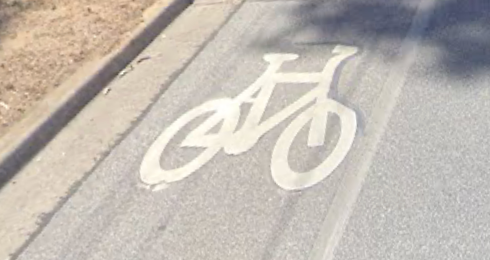
\includegraphics{f001_symbol.png}
\caption{Example bicycle lane marking.  Source: Google Street View, Oct 2019}
\label{fig:symbol}
\end{figure}

This marking is universal across all standard bicycle lanes in Australia, and can distinguish a bicycle lane from other types of road segment.  It may sometimes appear on a green surface, and occasionally it may be partially occluded due to limited space or wear and tear.  Similar markings exist in many other jurisdictions outside Australia.

In order to train a deep learning model to recognise bicycle lane markings in street scene images, it was necessary to first create a dataset of labelled images for training and validation.  This could then be used to apply a variety of pre-trained models from the ``TensorFlow 2 Model Garden'', through a process of transfer learning.

\subsection{Gathering a training dataset of Google Street View images}

The official Australian design standards for bicycle lanes specify that bicycle lane markings should appear within 15m of each intersection \cite{standards}.  Therefore, intersections along known bicycle lane routes are the most likely locations to find example images.

Campbell et al., 2019 \cite{CAMPBELL2019101350} successfully trained a deep learning model to recognise ``Stop'' and ``Give Way'' signs with 500 example images of each.  Therefore, an initial dataset of 500 bicycle lane marking images was gathered, with an option to gather more images if necessary.

A Jupyter Notebook took was created to allow an operator to efficiently review Google Street View images from intersections along known bike paths, and record which image files included examples of a bicycle lane marking.  The matching images could then be ``labelled'', to record the precise bounding box around each bicycle lane marking found in the images, in a format suitable for the TensorFlow 2 framework.

\subsubsection{Identifying candidate intersections to sample}
\label{s:sample_candidates}

Two candidate sources of information about ``known'' bicycle lane routes were considered for use in the sampling process:  The ``Principal Bicycle Dataset'', and XML extracts from the OpenStreetMap database.  These datasets are discussed in detail in section \ref{s:datasets}.  The ``Principal Bicycle Network'' dataset was chosen, partially because it is the incumbent official dataset, and partially due to its age.  If it was last updated several years ago, then there is a much lower risk of attempting to sample an intersection, only to find that the bicycle lane was constructed too recently to appear in the available Google Street View data.  However, the approach of using OpenStreetMap as a source of ``known'' bicycle routes to drive the sampling would have the advantage that it generalises to other jurisdictions, and it ultimately proved to be less complex.  Tools were created to generate lists of candidate intersections to sample in Google Street View for both approaches.  For instructions on how to operate the tools, please refer to Appendix \ref{a:sample_pbn} and Appendix \ref{a:sample_osm}.

Working from an XML extract of the OpenStreetMap database is the simplest approach.  Data can be downloaded for an individual country via \url{https://download.geofabik.de} and then sliced into a smaller area, if necessary, using the ``osmium'' command line tool from \url{https://osmcode.org/osmium-tool/}.  For more background on concepts in the OpenStreetMap data, please refer to Appendix \ref{a:osm_concepts}.  Briefly, an OpenStreetMap XML extract file contains ``ways'', which usually represent road segments, and ``nodes'', which represent strings of coordinates that make up the ``ways'' and thereby describe the ``shape'' of the ``way'' on a map.  If a ``way'' may have a number of ``tags'' attached to it, to record its characteristics.  If a contains a ``cycleway'' tag, then it has a bicycle lane.  If a ``node'' is common to multiple ``ways'' with different names, then it is an intersection.  A list of candidate intersections along ``known'' bicycle lane routes can be extracted exclusively from OpenStreetMap XML data, as follows:

\begin{itemize}
\item{Use the ``osmium'' tool to reduce an OpenStreetMap database file for a country, from \url{http://download.geofabrik.de}, down to the required area.  The tool can either reduce the map to a required bounding box, or it can be asked for data about an arbitrary shape, based on official geographic boundaries for a town or Local Government Area specified in a .geojson file.}
\item{Load the OpenStreetMap XML data into memory.  Find all ``way'' objects that are tagged as having a ``cycleway''.}
\item{For each way with a ``cycleway'', check every ``node'' in the way.  If the node is found in any other ``way'' that is a road but has a different name, then the ``node'' is an intersection.  Include the ``node'' ID and its coordinates in the list of candidate intersections to sample.}
\end{itemize}

Working from the ``Principal Bicycle Network'' dataset is more complicated, because although it describes the shape of each bicycle lane route in .geojson format, it does not have any information about intersections.  The data must be matched to OpenStreetMap to list the intersections along each route.  Another significant limitation is that it does not always list the name of the road for each bicycle lane route, and it never lists the town or suburb.  To overcome these limitations, the following approach was taken:

\begin{itemize}
\item{Explode each `Principal Bicycle Network'' dataset record into a list of coordinates.}
\item{For each coordinate, use a ``Nominatim'' server instance to determine the name of the road and the town or suburb, via a ``reverse-geocoding'' API call.}
\item{For each coordinate with a named road and town/suburb, use an OpenStreetMap XML extract of the general area to identify ``ways'' with a matching name, and then look up all intersections.  Use a bounding box around the original route coordinates from the ``Principal Bicycle Network'' dataset to exclude streets in the OpenStreetMap data that just happen to have the same name, in another town.  E.g. ``Main Street'' might occur in many towns across Victoria.}
\end{itemize}

A local instance of ``Nominatim'' was installed and used for this purpose, because the terms of use for public instances discourage bulk operations and limit them to one per second.  It was set up on a local machine as per Appendix \ref{a:computer}, following the official instructions \cite{nominatim_install}.  The instance was loaded with data for Australia only, onto solid-state disk.

Once intersections were identified from the OpenStreetMap data, it proved to be helpful to also calculate an approximate heading along the bicycle lane route at each intersection, to ensure that Google Street View images could be requested with the camera facing in a sensible direction.  The Python "geographiclib" library can calculate a heading from one point to the next.  Therefore the heading at each intersection was calculated to be the average of the heading from the previous ``node'' on the ``way'' to the intersection ``node'', and the heading from the intersection 	``node'' to the next ``node''.

\subsubsection{Downloading sample Google Street View images for the training dataset}
\label{s:sample}

Google provides an API for downloading Google Street View images of up to 640x640 pixels, at a cost of \$7.00 USD per 1,000 images.  Volume discounts are available, with a reduced cost of \$5.60 USD per 1,000 image for volumes from 100,001 to 500,000 images, and beyond that, further volume discounts can be negotiated with Google's sales team \cite{gsv_billing}.

The Python ``\texttt{google\char`_streetview}'' library was used to facilitate access to this Google Street View API from Python code.  In order to minimise costs, whenever an image was downloaded via the API, a copy of the image and its associated metadata was cached locally at a path that depended on the request parameters.  If a request was made for the same image at a later date, it would be retrieve from disk instead of issuing a further request to Google, to minimise costs.

The Google Street View API allows images to be requested for a location (latitude/longitude) with a desired heading, field-of-view angle, and camera angle relative to the ``horizon''.  A Jupyter Notebook was created to:

\begin{enumerate}
	\item{Select a sample location and heading from a CSV of candidate intersections.}
	\item{Download four Google Street View images at 0, 90, 180, and 270 degrees relative to the desired heading, with a 90 degree field of view for each image, and the camera angled 30 degrees towards the ground to focus on any nearby road markings.}
	\item{Allow the operator to quickly record which of the four images they see a bicycle lane marking in to a CSV file, so that it can be saved to a list of images to be labelled and included in the training dataset.}
	\item{Repeat.}
\end{enumerate}

It was found that the best location to look for a bicycle lane marking was not always right in the middle of an intersection, especially for large intersections.  Therefore, the option was added to allow the operator to ``browse'' a desired number of metres before or after the intersection, along the route heading, to find a good image.  If a bicycle lane marking appeared at the intersection, typically it could be found within 20-30m, except for major intersections with bicycle lanes that are terminated by turning lanes.

Generally, an image was accepted for inclusion in the training dataset if the bicycle lane marking clear enough to be unambiguous without taking cues from the overall scene context.  The shape of the bicycle in the marking had to be visible.  If the symbol was so far away that it looked like a white blob on the road, and could only be understood to be a bicycle lane marking by looking at how it was placed relative to lane markings, then the image was not included, though the operator had the option of moving the camera closer to it for a better image.

The Jupyter Notebook allowed multiple candidate intersections to be assessed per minute, and an initial set of 500 images was collected over the course of approximately 4 hours.

Please see Appendix \ref{a:download_gsv} for detailed instructions on how to use the supplied Jupyter Notebook to download Google Street View images for sample candidate intersections, and flag matching images in an output CSV file for inclusion in the labelled training dataset.


\subsubsection{Labelling the training dataset}
\label{s:label}

Once a suitable number of Google Street View images containing bicycle lane markings were collected, they were copied to a folder and then labelled using the open-source tool "labelImg" \cite{labelImg}.  Please refer to the tool's official documentation for installation and usage instructions.  The output of the tool was an XML file corresponding to the each original image file in the folder, in a format that could be understood by TensorFlow 2 training tools and scripts.

\subsection{Training and evaluating candidate models from the TensorFlow 2 Model Garden}

Training and evaluation of candidate models was conducted on local infrastructure, as described in Appendix \ref{a:computer}.  This task could also be performed on cloud-based infrastructure such as Google Collab, if required.  For general directions on how to set up a local computer to enable TensorFlow machine learning that takes advantage of GPU acceleration, please see Appendix \ref{a:setupenv}, or find the latest tutorials and guides online.

The training dataset that was collected in section \ref{s:sample} and labelled in section \ref{s:label} was randomly split into ``training'' and ``testing'' datasets according to an 80:20 ratio, using a ``bash'' shell script.

A Jupyter Notebook was used to set up the experiment, by transforming the labelled image datasets into TensorFlow records, downloading and configuring a pre-trained model from the TensorFlow 2 Model Garden, and creating scripts to train and evaluate the model.

The performance of each model depended on three key factors that could be adjusted:

\begin{itemize}
\item{The size of the dataset available for training.}
\item{The number of epochs spent training, where an ``epoch'' is a training iteration where a complete pass is made over the training dataset.}
\item{The threshold confidence score, from 0\% to 100\%, at which the model assumes that a bicycle lane marking has been detected.}
\end{itemize}

The initial size of the dataset was set based on previous experience in other papers such as Campbell et al., 2019 \cite{CAMPBELL2019101350}, with the option to extend it later if necessary.  In practice, it was found that the initial size was sufficient to obtain extra results for detections from Google Street View images, and no further training images were required.

During the training process, the TensorFlow training script showed ``loss'' performance metrics every 100 epochs.  The performance reported by the training script gradually improved as more training was conducted over the dataset.  Every few thousand epochs, training was paused, and an evaluation script was run to test the performance of the model against the independent testing dataset that had been withheld from the training process.  When training reached the point that further epochs did not significantly improve performance in either the training or the evaluation, training was halted.

As part of the evaluation process, image files were written to disk, containing the original image with an overlay where the bounding boxes and confidence score of any detections were drawn.  These were examined to determine how many false positives and false negatives there were, and the confidence scores when the model returned any false result.  The threshold confidence score was tuned in response to these findings, to find as many true positives as possible without significant numbers of false positives that might cause bicycle lane routes to be ``detected'' where they do not really exist.

The boundary boxes of detections were also checked to ensure that the results were sensible.

Multiple pre-trained models from the TensorFlow 2 Model Garden were trialled, with selections guided by their advertised ``Speed'' and ``COCO mAP'' (mean Average Precision) metrics.  The process of building a map of bicycle lanes for an area can be considered a ``batch'' process, with no fixed time constraints, therefore Mean Average Precision was prioritized over speed.

Please refer to Appendix \ref{a:tensorflow_training} for detailed instructions on how to reproduce the training process.

% ~~~~~~~~~~~~~~~~~~~~~~~~~~
\section{RQ2: Building a map of bicycle lane routes from Google Street View images in an area}
\label{s:rq2}

In section \ref{s:rq1}, a model was trained to detect bicycle lane markings in a single street view image.  To generate a map or dataset of bicycle lanes in an area, the first step is to determine a list of locations for which Google Street View images should be downloaded and processed by the model.  A batch process is then used to process each image and record whether a bicycle lane marker was found.  Finally, the list of sample locations where there was a ``hit'' must be correlated to geospatial data about the road network to infer  routes and draw them on a map.

\subsection{Sampling strategy for Google Street View images}
\label{s:rq2a}

In section \ref{s:sample}, it was noted that Google currently advertises a minimum cost of \$7.00 USD per 1,000 Google Street View images, and that the most likely place to find a bicycle lane marker is in the area immediately surrounding an intersection.  It was also found that the Google Street View API would only return distinct images every 10 metres.  Two sampling strategies were considered:
\begin{itemize}
\item{Generating a list of sample points every 10 metres along every street in the area.}
\item{Generating a list of sample points within a configurable distance of each intersection in the area, at 10 metre intervals.	}
\end{itemize}

Depending on the density of intersections in an area, limiting the samples to the immediate area around intersections could result in a significant cost reduction.  The ``intersection'' strategy was chosen, with the option to switch to full 10 metre sampling strategy if the results showed that too many bicycle lanes were being missed where they might otherwise have been detected with more samples.

An OpenStreetMap XML extract file for the area was loaded into memory and used to iterate over all streets and intersections in the area, resulting in a CSV batch file of sample locations to be downloaded from Google Street View and processed by the model.  The size of the batch file was inspected to assess potential cost before proceeding with the download from Google Street View.

When loading and interpreting the OpenStreetMap XML extracts, it was important to understand that while a ``way'' object in the data typically represents a road segment, but it may also represent the boundary of a reserve, a natural feature such as a coastline or creek, or a walking trail.  To avoid unnecessary requests to the Google Street View API for off-street locations, it was necessary to inspect the ``tags'' associated with each ``way'' to isolate actual road segments.

Another important consideration was how to handle roads that form the boundary of the area being surveyed.  If ``osmium'' is used to create an OpenStreetMap XML extract for a precise area according to a ``shape'' .geojson file describing its official boundary, then the resulting extract may exclude intersections where the intersecting road exists entirely outside the boundary.  This problem was addressed by allowing the operator to load a second OpenStreetMap XML extract file to cover a 200 metre margin around the area being surveyed.  Streets in the margin would not be considered in the survey for possible bicycle lane routes, but sufficient information was loaded from the second file to identify any roads that intersect the survey area at the margins.

Once the sample process has been run, the output is a CSV to document the coordinates of each point that needs to be downloaded from Google Street View and examined.  The CSV file includes additional columns to record the OpenStreetMap ``way'' ID and ``node'' ID associated with each point, so that any results can be linked back to the map.  Other fields such as the street name were also included for traceability.

Please see Appendix \ref{a:sample_area1} for detailed instructions on how to operate the tool that was used to generate a list of sample locations.


\subsection{Batch processing of Google Street View images}
\label{s:rq2b}

Once sample locations have been selected and recorded in a CSV file, a batch process works through the list, downloading any Google Street View images that have not already been cached locally.  Then, the selected deep learning detection model is called to process each image in turn.  If one or more bicycle lane markings are detected in an image, a copy of the image is saved to a folder of ``hits'', with the bounding box and confidence score included in the image to show where the detection was found.  A record is also inserted into a CSV file of detection locations.  If no bicycle lane marking is found in the image, a copy is instead placed in a separate ``miss'' folder.  Partitioning result images into separate  ``hits'' and ``misses'' folders allows the operator to quickly browse the images to check for any false positives or false negatives.

\remark{FIGURE: detection image for GSV}

Please see Appendix \ref{a:gsv_batch} for detailed instructions on how to operate the tools to download and cache Google Street View images for a list of sample locations, then process them with the model.


\subsection{Converting detection points into bicycle lane routes on a map}
\label{s:rq2c}

The result of the previous batch process in section \ref{s:rq2b} is a list of locations where a bicycle lane marking was found, linked back to the OpenStreetMap ``way'' IDs and ``node'' IDs that they were sampled from.  The next step is to convert these detection points into contiguous routes that can be drawn as lines on a map.

Google Street View image samples were taken 0, 90, 180, and 270 degrees from the assumed heading at each point, to provide to provide 360 degree coverage.  This allows detection of bicycle lane markings not just in the the forward and rear views, but also close alongside the camera vehicle, to improve the chances that an image will be found where the marking is clearly visible.  The detection model has been trained to detect markings in any orientation, and many of the samples will be taken at intersections.  Therefore, when drawing routes, proper consideration must be made about whether a detection belongs to the route being inspected, or an intersecting street.

Routes were inferred from the individual detection points based on the assumption that if markings were detected at two or more consecutive intersections along a named road, there is a bicycle lane along that segment.  A configuration option was provided to allow for one or more intersections without  detections before assuming that the bicycle lane route route has been interrupted.

A continuous road may be divided up into multiple ``way'' segments in the OpenStreetMap data if any of its characteristics change from one segment to the next, such as the speed limit dropping for school zones.  Before inferring bicycle lane routes along a road from the detection points, it was necessary to link adjacent ``way'' segments from a single named road back up into a single chain.

Each inferred route was written to a .geojson file as a ``LineString Feature'', following the original co-ordinates of all ``nodes'' in the original OpenStreetMap data, from start to finish.


\subsection{Comparing results to other data sources}

Once a .geojson file has been produced to describe the detected bicycle lane routes, it can be drawn on a map in a Jupyter Notebook using the Python ``ipyleaflet'' library.

The total length of all routes in a .geojson file can be calculated by using the Python ``geographiclib'' library to calculate the distance between each pair of points along the route.

The OpenStreetMap XML extract for the survey area can be used to generate an equivalent .geojson file of bicycle lane routes according to OpenStreetMap.  The data is filtered down to ``ways'' that are roads and that have a ``cycleway'' related tag.  Then a ``LineString Feature'' is written to an output .geojson for each cycleway.

The detected routes .geojson file and the OpenStreetMap-derived .geojson file can be drawn on maps side-by-side for visual comparison, and the differences can be measured at a high level by comparing the total length of the routes in each file.

To drill down further into the detail of the differences, multiple .geojson files were created:

\begin{enumerate}
\item{A .geojson file with all bicycle lanes from the detection model}
\item{A .geojson file where a bicycle lane was detected that was not recorded in OpenStreetMap}
\item{A .geojson file where a bicycle lane was recorded in OpenStreetMap but not detected}
\item{A .geojson file where both the detection model and OpenStreetMap agree that there is a bicycle lane}	
\end{enumerate}

Items 2-4 can be drawn as layers on a single map, each with their own color, to highlight where the bicycle lanes are, and where they disagree.  By measuring the distances in the file, we can quantify how much agreement there is between the two sources, and how many metres worth of bicycle lane routes are in one but not the other.

Where there is a disagreement between the output of the detection model and what has been recorded in OpenStreetMap, the original images or footage can be reviewed to establish the truth, and whether the detection model was producing reasonable results for the input.

The ``Principal Bicycle Network dataset'' is available in a .geojson format.  A quick visual comparison is therefore possible, by drawing it on a map side-by-side with the .geojson file of detected bicycle lane routes.  To quantify the differences in more detail:

\begin{enumerate}
\item{For each point in the Principal Bicycle Network dataset .geojson file, find the closest point in the OpenStreetMap XML extract and its ``node'' ID.  Exclude any points outside the bounding box of the survey area.}
\item{Use the coordinates of the matching ``node'' from the OpenStreetMap data, instead of the original coordinates from the Principal Bicycle Network dataset, to ensure that the sources are ``aligned'' on a common understanding  of where the road network is.}
\item{Produce four output .geojson files to compare the ``aligned'' Principal Bicycle Network dataset to the detected bicycle lanes, following the same basic process that was used for the OpenStreetMap comparison.}
\end{enumerate}


% ~~~~~~~~~~~~~~~~~~~~~~~~~~
\section{RQ3: Applying the process to dash camera footage}
\label{s:rq3}

The use of Google Street View images for detection of bicycle lanes has both advantages and disadvantages to consider.  Google Street View image data is readily available for a wide area across many jurisdictions internationally, and it can be collected without a physical presence on location.  However, usage comes at a cost, which may be a significant factor if mapping is required across a large area.  The image resolution is limited to 640x640 per image, though perhaps this limitation could be worked around by requesting many more images per location, each with a tighter field of view, at additional cost.  Distinct images appear to be only available every 10 metres.  The images may be several years out of date.  The position of the camera cannot be controlled, and might miss service roads or the other side of a divided road.  With only one image available for each location, a bicycle lane marking might be obscured due to bad luck.

A local authority might prefer to gather their own footage, to address these shortcomings.  For the third research question, we explore whether we could detect bicycle lane routes from dash camera footage instead, perhaps taken from vehicles that must regularly traverse the roads in the area to provide other services, such as waste disposal or delivery trucks.


\subsection{Choice of dash camera hardware}
\label{s:rq3a}

For these experiments, the ``Navman MiVue1100 Sensor XL DC Dual Dash Cam'' was self-installed inside a passenger sedan a typical location behind the rear-view mirror, at a cost of \$529 AUD.  This model was selected because for each one minute of footage recorded in an MP4 video file, it also records an NMEA file with latitude, longitude, heading, and altitude at one second intervals.  The NMEA metadata allows each frame in the footage to be linked to a location, by correlating the frame number to nearest NMEA measurements, and extrapolating readings across the 1 second interval as required.

Video footage was recorded at 60 frames per second, at 1920x1080 resolution.

The camera features a ``wide angle'' lens to capture a good view of the road and its general surroundings, however exact specifications such as focal length were unknown.


\subsection{Gathering and processing dash camera footage}
\label{s:rq3b}

On the 3rd of October, 2021, Melbourne set the record for the longest ``COVID lockdown'' in the world \cite{lockdown_record}.  Severe restrictions were placed on residents being more than 5km from home, gradually easing to 10km and then 15km \cite{lockdown_5km}.  Therefore it was only possible to experiment with dash camera footage from a confined area.

Approximately 100 minutes of footage was gathered by driving within a local area around the outer metropolitan suburbs of Mount Eliza, Frankston, Langwarrin and Baxter in Melbourne, Victoria, Australia.  Not every road in the area was covered.  Roads were selected for inclusion in the footage to include all known bicycle lanes in the area, based on local knowledge and a review of the OpenStreetMap data.  A variety of other roads were included, to cover roads with and without a paved shoulder, major divided roads and small local roads, and a mix of residential and commercial areas.

The dash camera video footage and corresponding NMEA files were transferred to a computer for processing via MicroSD card.  Then a batch process was set up in Jupyter Notebook to process each pair of files in a directory.

For each pair of files, the NMEA file was loaded into memory, then the video file was split into a series of images via the ``OpenCV'' library.  Reviewing the footage, it was decided that it was only necessary to process every 5th frame in order to get a clear view of every bicycle lane marking, effectively reducing the footage from 60 frames per second to 12 frames per second.  The latitude, longitude, altitude, and heading for each frame was calculated or extrapolated from the NMEA records.  Each frame was recorded to disk as a .png file for traceability, with a filename consisting of the original video filename, and a four-digit frame number.  Browsing these files in alphabetical order preserved their original chronological sequence.  For each frame, an entry was added to an output ``batch'' CSV file to record the path to the image file to be processed, and its associated location metadata.

The batch CSV file was processed by the detection model to yield another CSV file with detection results, as per the Google Street View process described in section \ref{s:rq2}.  For images where at least one ``BikeLaneMarker'' was detected, a copy of the image with a green bounding box was written to a ``hits'' directory for manual inspection.  For images where a ``BikeLaneMarker'' was not detected, a copy was written to the ``miss'' directory.  Images in the ``hits'' and ``miss'' folders could be quickly inspected manually.


\subsection{Training the bicycle lane detection model}
\label{rq3c}

The dash camera footage was initially processed using the original model that was trained exclusively on Google Street View images in section \ref{s:rq1}, without any retraining based on dash camera images.  The original model was able to detect every bicycle lane marking in the test footage, however further training and refinement was required to address some performance issues:

\begin{itemize}
\item{Although the Google Street View-trained model was able to detect every marking, it typically only did so when the marking was very close to the car.  Further training was needed on footage from the dash camera in order to allow it to detect markings that were further away, but still close enough to be clearly visible.}
\item{There were also issues with false positives that had not been apparent when using the Google Street View model on Google Street View images.  The model would sometimes yield false positives for the following:

	\begin{itemize}
	\item{Short white dashes painted at intersections to advise drivers to give way}
	\item{White arrows drawn on the road surface, such as turning lane arrows}
	\item{Diagonal white stripes that were drawn on the road to represent traffic islands}
	\item{Large white writing on the road, such as ``KEEP CLEAR''}
	\item{Pale road defects and anomalies}
	\item{Reflections from the bonnet of the camera vehicle}
	\item{Random objects well outside the boundary of the road}
	\end{itemize}
}
\end{itemize}

A decision was made to train the model with selected images from the half of the footage that was gathered in Frankston, Langwarrin, and Baxter, and to test on the independent images gathered in Mount Eliza.  The footage from this new training areawas processed through the original Google Street View-trained model to identify \remark{HOW MANY?} images with true positives and false positives.  These images were then selected for labelling, to be added to the training and validation data.

The original Google Street View training images had been labelled with a single class ``BikeLaneMarker''.  The new training images selected from dash camera footage of the training area were labelled with additional classes, to encourage the model to think of them as something other than a bicycle lane marker:

\begin{itemize}
\item{BikeLaneMarker}
\item{GiveWayMarker}
\item{ArrowMarker}
\item{IslandMarker}
\item{RoadWriting}
\item{RoadDefect}
\end{itemize}

Once these new images had been labelled, they were randomly split 80:20 and added to the Google Street View images in the original training and testing datasets.  The models were then re-trained from scratch based on the combined training dataset, and tested against thew new combined test dataset.

To deal with the false positives that had triggered by reflections on the bonnet of the camera vehicle, and random objects on the side of the road, the process was updated to apply a mask to each image before passing it to the detection model.  The mask was designed to exclude the bonnet of the vehicle and anything on the opposite side of the road, and focus attention on places in the frame where a bicycle lane marker might reasonably be encountered in the direction of travel.

\remark{a picture would be nice}

The detection model that had been re-trained to include dash camera images from the training area of Frankston/Langwarrin/Baxter was then evaluated against the independent footage from the Mount Eliza area.


\subsection{Mapping dash camera detections and comparing to other sources}
\label{s:rq3d}

Processing a batch of images from the dash camera yields a CSV file with detection locations.  The location coordinates in these results came from NMEA file, and they may not exactly match ``node'' coordinates from the OpenStreetMap XML data extract.  To produce a map of bicycle lane routes detected from the dash camera footage, we first ``align'' the detection co-ordinates with ``node'' coordinates found in the OpenStreetMap data.  This allows us to more easily compare routes and measure the differences.

For every detection location logged by the model, we find the nearest ``way'' in the OpenStreetMap XML extract that belongs to a named road.  The Python ``shapely'' library helps us to perform this search as efficiently as possible, using bounding boxes for each way to avoid a brute force search of all points.  Once we have found the nearest ``way'', check every ``node'' in the way to record the nearest intersection ``node'', and the nearest ``node'' of any type.  We consider there to be a ``hit'' at the co-ordinates of both nodes:  The point on the OpenStreetMap route closest to the detection -- which may a bicycle lane marking that occurs at regular intervals of up to 200 metres along the road \cite{standards} -- and the closest intersection along the road.

Once the detection coordinates have been aligned to the OpenStreetMap coordinates, .geojson files can be ``drawn'' and compared to other sources using the same techniques as for the Google Street View images.  This process is based on the nearest intersection for each detection, but preserving the co-ordinates of the nearest ``node'' of any type in the output helps with traceability.


% ~~~~~~~~~~~~~~~~~~~~~~~~~~
\section{RQ4: Surveying other infrastructure details using dash camera footage}

Once dash camera footage had been used to map bicycle lane routes in a survey area, some further work was conducted to demonstrate how the approach might be re-used to survey other details of interest.  To demonstrate future potential, a process was created to map any paved shoulders on the side of the roads in the survey area that cyclists might ride on achieve physical separation from motor vehicles.  Previous studies such as Klobucar \& Fricker, 2007 \cite{BIKESAFETY} have observed that a paved shoulder can improved cyclist safety, even if it is not formally marked as a bicycle lane.

For a discussion of other areas of potential for future work, please refer to section \ref{s:future_work}.

To identify a paved shoulder, it is necessary to detect lane markings, and the edge of the road if it is not explicitly marked.  We are interested in the edge of the road on the side of the road that traffic usually drives on.  In this research, dash camera footage was captured in Australia, so we are interested in the left hand side.  The following section therefore refers to the ``left''.


\subsection{Correcting for lens distortion}

Lens distortion is where the optical properties of a camera's lens causes straight lines to appear curved in an image.  The ``OpenCV'' library provides a method to correct distortion for a specific camera \cite{distortion}.  The camera is used to capture a range of images where a special calibration tool appears in frame.  Then a the series of images is used to create a mathematical model of the camera's lens distortion.  Once this model has been created, it can be used to apply a transformation to any image from the camera in question.

\remark{see demo figures showing the calibration process}

When searching for paved shoulders in a survey area, we are looking for lines in an image that are often straight.  The dash camera being used to collect images was therefore calibrated, and images processed to correct for distortion in this part of the exercise, in case the distortions had an impact.  This operation may also be assist future work to estimate the width of detected lanes.

\remark{see demo before and after images}


\subsection{Detecting lane markings}

A common solution to the problem of detecting lane markings involves applying a combination of the Canny edge detection algorithm proposed by Canny, 1987 \cite{canny} and the Hough transformation proposed by Hough, 1972 \cite{hough}.  This general approach has been followed in many papers such as  Li et al, 2016 \cite{canny_example} or Chai et al, 2014 \cite{canny_example2} and it is frequently used in capstone projects in the self-driving car domain.  At its most basic, the approach does not involve any machine learning or deep learning techniques.

The Canny/Hough approach typically works as follows:

\begin{itemize}
\item{Apply Canny edge detection to detect edges in an image \cite{canny}}
\item{Apply a mask to exclude edges outside a triangle representing the area immediately in front of the vehicle}
\item{Apply a Hough transform \cite{hough} to convert these edges into lines, each line having a slope and an intercept.}
\item{Partition the lines into two groups:  Lines that slope upwards from left to right, and lines that slope downwards from right to left.}
\item{For each group of lines, take the average slope and intercept.  These represent the detected lane boundaries.}
\item{Use the slope and intercept of each detected line to overlay a line on the original image, extending from the bottom of the image to a suitable ``horizon'' somewhere around half-way to the top of the image.  These straight lines allow visualization of the detected lane boundaries.}
\end{itemize}

Please see figure \remark{I really want a figure demonstrating each stage!}

The ``OpenCV'' library provides convenient tools to implement the required transformations.

Typically, the process is used to detect the camera vehicle's own lane.  In order to detect a paved shoulder, we first want to detect the boundaries of our vehicle's own lane, then perform a second pass at the image where the mask has shifted to focus exclusively on areas to further to the edge of the road.

\remark{Create sample images and include them and refer to them to explain this better.}

A detected paved shoulder will be defined by two lines, each with a ``slope'' and an ``intercept''.  One line will be the left boundary of the camera's own lane, which is also the right boundary of the paved shoulder.  The other lane will be the left boundary of the paved shoulder, further to the edge of the road.  In the following example images, the detected lines have been overlaid  on the original image, along with two horizontal intersection lines.  The lower horizontal line is intended to show an intersection as close as possible beyond the bonnet of the camera vehicle, and the upper horizontal line is further into the distance, towards a ``horizon''.

If the Canny/Hough approach cannot find another line to the left of our the camera vehicle's own lane, it is a strong sign that there is no clearly defined paved shoulder on the road at that location.  If a line is found, it could be a paved shoulder, or it could be a false positive caused by ``noise'' from something beside the road.  Please see figures \remark{here} for examples of true positive and false positive detections.  The potential for ``noise'' from false positives should be taken into account when attempting to create a map of paved shoulders across the survey area.

\remark{obvious true positive, obvious true negative, sketchy false positive}

roads only
30m from intersections
prop missing
intersection y std => find intersection (x,y) of the intersection of the lines
intersection x std
width top mean

\subsection{Mapping paved shoulders across a survey area}

The Canny/Hough lane detection method can be applied to all sample frames from the survey area, by using a similar batch process to the bicycle lane detection process in section \ref{s:rq3} and substituting a different detection model.  The challenge is setting robust criteria for flagging a ``detection'' that will result in a sensible map.  The simplest criteria would be to look for frames where lines were detected for both the left and right boundaries of a paved shoulder.  This criteria was applied to the Frankston/Langwarrin/Baxter training area footage, and the resulting images with detection line overlays were reviewed in chronological order.  The results were very inconsistent.

Reviewing the footage, it was found that on roads where there was a paved shoulder or bicycle lane, the boundaries of that lane remained relatively stable from frame-to-frame, and the width of gap between the boundaries towards the ``horizon'' at the top of the frame was relatively wide.  There were relatively few ``skipped'' frames where the boundaries were not detected.  In contrast, on roads without a paved shoulder or bicycle lane, there may be many ``skipped'' frames, the slopes of the detected boundaries were much less consistent from frame-to-frame, and the detected boundary lines often had an intersection point much closer to the bottom of the frame.

The following solution was proposed:

\begin{itemize}
\item{Each frame would be linked to its two nearest intersection ``nodes'' in the  OpenStreetMap data.  Frames associated with a single stretch of road between two intersections would be assessed as a group, to determine whether a paved shoulder or bicycle lane exists along that stretch.}
\item{Frames from locations within 30 metres of an intersection were excluded from consideration, because it is common for them to ``disappear'' at the approach to an intersection, and this disappearance should not counted as a missed detection.}
\item{If the model fails to find both boundaries of a paved shoulder in more than 20\% of the remaining frames along a stretch of road, then it is assumed that there isn't one.}
\item{A horizontal line is drawn across the frame towards a ``horizon'' as per figure \remark{REF}.  The width of the space between the boundary lines is measured at this height within the frame, in pixels.  The mean width is calculated across all frames in the stretch of road where boundary lines were detected.  If the mean is less than 75 pixels, then the possible paved shoulder is too narrow, and it is assumed not to exist.  This accounts for very narrow margins such a gutter that are of no use to a cyclist.}
\item{If the model finds both left and right boundary lines for a possible paved shoulder, use the slopes and intercepts to calculate an (x,y) coordinate relative to the bitmap image where those two boundary lines intercept.  Calculate the standard deviation of the x and y intersection values across all frames in the stretch of road where both boundary lines are defined.  If the standard deviation in either the x or y dimension is greater than 50 pixels, then the boundary lines are considered to be too inconsistent.  The stretch of road is assumed not to have a paved shoulder.}
\end{itemize}

The thresholds described above were set based on the following process:

\begin{itemize}
\item{Update the batch process to output a row for every frame, in chronological order}
\item{Include the name of the road for traceability.}
\item{Include the node IDs of the two nearest intersections, to trace which frames are part of the same group.  The first node ID is the one that comes first alphabetically, not the one that is closest to the location associated with the frame.  This is to avoid splitting a group of frames for a stretch of road into two groups depending on which intersection is closest.}
\item{Filter out frames where the location is within 30m of either of the two nearest intersections}
\item{Create summary statistic columns for each group for frames, and add them to the output CSV as additional columns:
	\begin{itemize}
	\item{Proportion of frames where boundary lines were not detected}
	\item{Mean width of the potential paved shoulder, in pixels, at the horizontal ``horizon'' line}
	\item{Standard deviation of the y-coordinate where the boundary lines intersect}
	\item{Standard deviation of the x-coordinate where the boundary lines intersect}
	\end{itemize}
}
\item{Apply this process to the training area footage from Frankston/Langwarrin/Baxter to produce an output CSV.}
\item{Load the output CSV file into an editor, and add a ``truth'' column to denote whether a paved shoulder really exists at each location, based on a review of the output frames with the detection line overlay.}
\item{Filter the data to find thresholds in the summary statistics that appear to explain how the ``truth'' values are partitioned, as closely as possible.}
\item{Create ``prediction'' column in the output CSV based on the chosen thresholds, and compare it to the ``actual'' value in the ``truth'' column.}
\end{itemize}

The model was then applied to the footage from the Mount Eliza testing area to see how it performed with the selected thresholds.

To construct a map of detected paved shoulders, take the distinct combinations of ``way'' ID and the ``node'' IDs of the two closest sections, where a paved shoulder was predicted.  Find the ``way'' ID in the OpenStreetMap data, and ``draw'' a ``LineString Feature'' in a .geojson file for all ``nodes'' between the two intersection nodes, including the intersection nodes themselves.  The .geojson file can then be drawn on map in a Jupyter Notebook using the Python ``ipyleafelet'' library as per sections \ref{s:rq2} and \ref{s:rq3}.


%%%%%%%%%%%%%%%%%%%%%%%%%%%%%%%%%%%%%%%%%%%%%%%%%%%%%%%%%%%%%%%%%%%%%%
\chapter{Results and Discussion}
\label{s:results}

\remark{Criteria 40: clear and complete presentation of results}

\remark{Criteria 40: sufficient quantity of work}

\remark{Criteria 40: appropriate intellectual level}

\remark{Criteria 40: appropriate consideration of evidence in discussion}

\remark{Criteria 40: uncertainty/error analysis}

\section{Opportunities for future research}
\label{s:future_work}

xxx


%%%%%%%%%%%%%%%%%%%%%%%%%%%%%%%%%%%%%%%%%%%%%%%%%%%%%%%%%%%%%%%%%%%%%%
\chapter{Conclusion}

\remark{Criteria 15: conclusions are supported by the observations/results/calculations}

\remark{Criteria 15: conclusions relate to the original research questions/aims/hypotheses}

%%%%%%%%%%%%%%%%%%%%%%%%%%%%%%%%%%%%%%%%%%%%%%%%%%%%%%%%%%%%%%%%%%%%%%
\appendix
\chapter{Computer Environment}
\label{a:environment}

Two computers were used

\section{Machine Learning workstation}
\label{a:computer}

xxx

\section{Nominatim server}
\label{a:nominatim}

xxx

\chapter{Identifying candidate intersections to sample based on cycleways in an OpenStreetMap XML extract}
\label{a:sample_osm}

xxx

\chapter{Identifying candidate intersections to sample based on existing bicycle lanes in the Principal Bicycle Network dataset}
\label{a:sample_pbn}

xxx

\chapter{OpenStreetMap concepts}
\label{a:osm_concepts}

xxx

\chapter{Downloading and flagging sample Google Street View images for the training dataset}
\label{a:download_gsv}

xxx

\chapter{General directions on setting up a local TensorFlow 2 development environment}
\label{a:setupenv}

xxx

\chapter{Training and evaluating a Deep Learning model from the Tensorflow 2 Model Garden}
\label{a:tensorflow_training}

xxx

\chapter{Sampling Google Street View images from a local area}
\label{a:sample_area1}

xxx

\chapter{Batch processing of Google Street View images}
\label{a:gsv_batch}

xxx

\chapter{Constructing a map from Google Street View detections}
\label{a:gsv_map}

xxx

\chapter{Applying model to Dash Camera footage}
\label{a:apply_dashcam}

xxx

\chapter{Detecting paved shoulders from Dash Camera footage}
\label{a:lane_detection}

xxx

\cleardoublepage
\bibliographystyle{IEEEtran}
\bibliography{Bib/references.bib}
\end{document}
\end{document}
